

在第一部门中先了解linux基础操作知识,他们包括系统知识,网络知识,


\chapter{系统基础}

\section{centos7 安装}

CentOS 7 网卡名不以eth0开始原因,是由于systemd 和 udev 引入了一种新的网络设备命名方式–一致网络设备命名(CONSISTENT NETWORK DEVICE NAMING) 。可以根据固件、拓扑、位置信息来设置固定名字,带来的好处是命名自动化,名字完全可预测,在硬件坏了以后更换也不会影响设备的命名,这样可以让硬件的更换无缝化。带来的不利是新的设备名称比传统的名称难以阅读。比如心得名称是enp5s0.

想要改为像centos6一样以eth0开始的名称有两种方法,在出现安装新系统的时候按下tab键,在kernel启动选项中增加 net.ifnames=0 biosdevname=0 

安装好后需要先做一些优化,fir

\begin{figure}[!ht]
    \centering    
    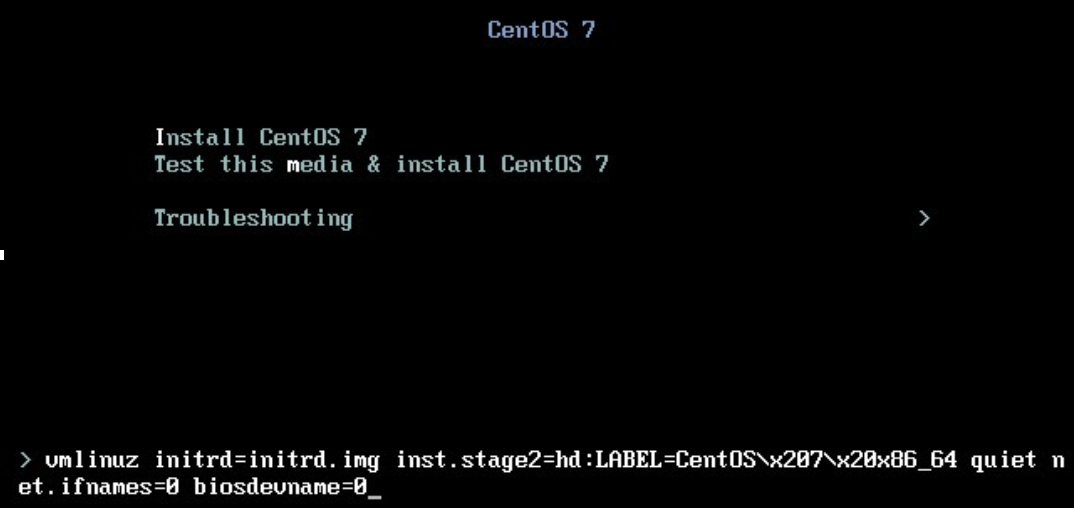
\includegraphics[width=0.8\textwidth]{linuxBasic/images/centos-bios.png}
    \caption{\label{Fig:async} Asynchronous I/O model}
\end{figure}

当然,如果在安装时忘记操作了也可以在启动后操作。在 /etc/sysconfig/grub下相应位置加上这两个参数,然后再改网卡名既可

\begin{lstlisting}
GRUB_CMDLINE_LINUX=”rd.lvm.lv=vg0/swap vconsole.keymap=us crashkernel=auto  vconsole.font=latarcyrheb-sun16 net.ifnames=0 biosdevname=0 rd.lvm.lv=vg0/usr rhgb quiet”

grub2-mkconfig -o /boot/grub2/grub.cfg

\end{lstlisting}

安装完系统后一般需要关闭selinux, NetworkManager, firewalld, 需要安装net-tools, lsof, tcpdump, epel,

\subsection{桥接}
一、网卡桥接设置:
\begin{itemize}
 \item 网卡配置文件:详见 ifcfg-enp8s0
\item 网桥配置文件: 详见 ifcfg-br0
\end{itemize}

二、网卡绑定设置:
\begin{itemize}
\item 网卡配置文件01:ifcfg-enp6s0f0
\item 网卡配置文件02:ifcfg-enp6s0f1
\item 网桥配置文件: ifcfg-bond0
\end{itemize}

3. 在bond0基础上增加多个桥接网卡
详情参见 ifcfg-bond0.300, ifcfg-virbr300;  ifcfg-bond0.3960, ifcfg-virbr3960

\section{磁盘分区与挂载}

\subsection{磁盘简介}
用于存储数据的物理设备便叫磁盘,磁盘接接口的不同可以分为:IDE,  SATA, SCSI, SAS.

\begin{itemize}
\item IDE的英文全称为“Integrated Drive Electronics”,即“电子集成驱动器”,
\item SCSI的英文全称为“Small Computer System Interface”
\item SATA(Serial ATA)又叫串口硬盘,PC机硬盘的主流趋势。
\item SAS(Serial Attached SCSI)即串行连接SCSI,是新一代的SCSI技术,此接口的设计是为了改善存储系统的效能、可用性和扩充性,并且提供与SATA硬盘的兼容性
\end{itemize}

磁盘内部由多个盘片,机械手臂,磁头,主轴马达组成。在读取数据时主轴马达驱动盘片转动,机械手臂可伸展来让磁头(head)读取数据,在盘片上存储数据,所以磁盘的容量便要看盘片的质量。

\begin{description}
	\item[磁道(Track)]:在每个盘片上由不同半经组成的同心圆叫做磁道,
	\item]扇区(Sector)]:每个磁道中被分隔成的最小的俱单位便是扇区每个扇区为512bytes
	\item[柱面(Cylinder)]:由多个盘片相同磁道所组成的圆柱面便是柱面
\end{description}

磁盘读取与写入数据时会按柱面来写入,只有柱面写完(读完)后才会切换磁道。
磁盘容量计算方式:Head * cylinder * Secor * 512bytes

每个磁盘的第一扇区非常重要,因为在该扇区存放着两个重要信息
1. 主引导分区(Master Boot Record, MBR) 有446bytes 主要用于安装引导加载程序
2. 分区表(Partition table) 记录整块磁盘分区状态,有64bytes

\subsection{磁盘分区}
由于分区表仅有64bytes所以只能记录4组记录区,每组记录区记录了该区段的启始与结束的柱面号码。所以每个磁盘只能分四个主(Primary)或扩展分区(Extended)。
而每个磁盘只允许有一个扩展分区,且扩展分区不能被格式化后存放数据,需要在扩展分区之上划分逻辑分区(Logical)。linux设备中的文件名1-4给主或者扩展分区预留,逻辑分区从5开始。

在linux下给磁盘分区的命令有`fdisk` 适合小于2T的磁盘分区, `parted` 擅长于大于2t 的磁盘分区。分区的实质便是修改分区表

\subsubsection{ fdisk 对磁盘分区}
使用命令`fdisk -cu /dev/sdb` 来进行对sdb分区,用命 -l来查看分区分区时的命令有

\begin{itemize}
\item  d   delete a partition 删除一个分区
\item  n   add a new partition       新增一个分区
\item  p   print the partition table 把分区打印出来
\item  q   quit without saving changes 不保存退出
\item  w   write table to disk and exit  保存分区并退出
\end{itemize}

这里需要注意在交互式分区过程中输错之后需要用**Ctrl + u**来撤消。 交互式实在太费事,这对于批量分区来说太费事可以用下面命令来一键搞定
\begin{lstlisting}
echo -e "n\np\n1\n\n+10G\nn\np\n2\n\n+20G\nw" |fdisk /dev/sdb
\end{lstlisting}

上一便仅是创建两个主分区,第一个分区给10G,第二个分区给20G,创建其它分区也类似

\subsubsection{ parted 对磁盘分区}
parted的操作都是实时的,也就是说你执行了一个分区的命令,他就实实在在地分区了,而不是像fdisk那样,需要执行w命令写入所做的修改, 所以进行parted的测试千万注意不能在生产环境中!
>传统的MBR(Master Boot Record)分区方式,有一个局限:无法支持超过2TB的硬盘的分区(或单个分区超过2TB)如果大于2T就要使用用GPT(Globally Unique Identifier Partition Table Format)分区的概念.

非交互式分区方式

\begin{lstlisting}
parted /dev/sdb  mklabel gpt yes
parted /dev/sdb  mkpart primary ext4 0 100  Ignore
parted /dev/sdb  mkpart primary linux-swap 101 8192 Ignore
parted /dev/sdb  mkpart logical ext4 8193 100GB  Ignore
parted /dev/sdb  mkpart logical ext4 101GB 3000GB Ignore
parted /dev/sdb  quit
\end{lstlisting}

\subsection{ 格式化与挂载}
磁盘分区好后,必须先格式化后才能挂载

\begin{lstlisting}
$ mkfs.ext4 /dev/sdb1
$ mkfs.ext4 /dev/sdb2

$ tune2fs -c -1 /dev/sdb1
tune2fs 1.41.12 (17-May-2010)
Setting maximal mount count to -1
#格式化后便可以挂载了
$ mount /dev/sdb1 /mnt
$ mount |grep --color=auto "/dev/sdb1"
/dev/sdb1 on /mnt type ext4 (rw)
\end{lstlisting}

在这里手动挂载后,系统重启后还需要再手动挂载一次,因为这里需要修改文件/etc/fstab 这个文件以达到开机自动挂载

磁盘被手动挂载之后都必须把挂载信息写入/etc/fstab这个文件中,否则下次开机启动时仍然需要重新挂载。 系统开机时会主动读取/etc/fstab这个文件中的内容,根据文件里面的配置挂载磁盘。这样我们只需要将磁盘的挂载信息写入这个文件中我们就不需要每次开机启动之后手动进行挂载了。挂载的限制
\begin{itemize}
\item  根目录是必须挂载的,而且一定要先于其他mount point被挂载。因为mount是所有目录的跟目录,其他木有都是由根目录 /衍生出来的。
\item  挂载点必须是已经存在的目录。
\item  挂载点的指定可以任意,但必须遵守必要的系统目录架构原则
\item  所有挂载点在同一时间只能被挂载一次
\item  所有分区在同一时间只能挂在一次
\item  若进行卸载,必须将工作目录退出挂载点(及其子目录)之外。
\end{itemize}

下面我们看看看/etc/fstab文件,这是我的linux环境中/etc/fstab文件中的内容

\begin{lstlisting}[language=bash]

$ cat /etc/fstab

#
# /etc/fstab
# Created by anaconda on Wed Oct 28 23:23:38 2015
#
# Accessible filesystems, by reference, are maintained under '/dev/disk'
# See man pages fstab(5), findfs(8), mount(8) and/or blkid(8) for more info
#
UUID=faba0886-9c24-430c-8ce5-f7980c283bbd /                       ext4    defaults        1 1
UUID=a2ea9c91-9424-4d8e-b15f-946ef8413877 /boot                   ext4    defaults        1 2
UUID=f11549e2-cd8a-4ec5-92ca-e8a83a16c87e swap                    swap    defaults        0 0
tmpfs                   /dev/shm                tmpfs   defaults        0 0
devpts                  /dev/pts                devpts  gid=5,mode=620  0 0
sysfs                   /sys                    sysfs   defaults        0 0
proc                    /proc                   proc    defaults        0 0
/dev/sdb1               /mnt                    ext4    defaults        0 0

\end{lstlisting}

可以看到fstab里一共有六列。

第一列 Device **Device**  是磁盘设备文件或者该设备的Label或者UUID
Label就是分区的标签,在最初安装系统是填写的挂载点就是标签的名字。可以通过查看一个分区的superblock中的信息找到UUID和Label name。
例如我们要查看/dev/sda1这个设备的uuid和label name
使用设备名称(/dev/sda)来挂载分区时是被固定死的,一旦磁盘的插槽顺序发生了变化,就会出现名称不对应的问题。因为这个名称是会改变的。不过使用label挂载就不用担心插槽顺序方面的问题。不过要随时注意你的Label name。至于UUID,每个分区被格式化以后都会有一个UUID作为唯一的标识号。使用uuid挂载的话就不用担心会发生错乱的问题了。

\begin{lstlisting}[language=bash]
$ dumpe2fs -h /dev/sda1
dumpe2fs 1.35 (28-Feb-2004)
Filesystem volume name:   /boot   #这个就是Label name
Last mounted on:
Filesystem UUID:          3b10fe13-def4-41b6-baae-9b4ef3b3616c    #UUID
Filesystem magic number:  0xEF53
Filesystem revision #:    1 (dynamic)
Filesystem features:      has_journal ext_attr resize_inode dir_index filetype needs_recovery sparse_super
Default mount options:    (none)
Filesystem state:         clean
#简单点的方式我们可以通过下面这个命令来查看
$ blkid /dev/sda1
/dev/sda1: LABEL="/boot" UUID="3b10fe13-def4-41b6-baae-9b4ef3b3616c" SEC_TYPE="ext3" TYPE="ext2"
\end{lstlisting}


第二列:Mount point 设备的挂载点,就是你要挂载到哪个目录下。

第三列: filesystem 磁盘文件系统的格式,包括ext2、ext3、ext3、reiserfs、nfs、vfat等. 生产场景中如果是大量小文件业务 首选 reiserfs。而 ext4 适合视频下载,流媒体,数据库,小文件业务

 ReiserFS是一个基于B状树的文件系统,拥有非常好的总体性能,特别是对于大量小文件。ReiserFS 拥有良好的伸缩性并具有日志功能。但该文件系统不再受到积极开发,不支持SELinux,基本上已被 Reiser4 取代。ReiserFS文件系统多年来一直用作一些发行版(包括SUSE)的默认文件系统,但现在用得少了。

 XFS文件系统拥有日志功能,包含一些健壮的特性,并针对可伸缩性进行了优化。XFS在RAM中强制缓存中转数据,因此如果使用 XFS,建议采用不间断电源供应。淘宝的数据库在使用此文件系统。

第四列:parameters 文件系统的参数

\begin{description}
	\item[Async/sync]设置是否为同步方式运行,默认为async
	\item[auto/noauto]当挂载mount -a 的命令时,此文件系统是否被主动挂载。默认为auto
	\item[rw/ro      ]是否以以只读或者读写模式挂载
	\item[exec/noexec]限制此文件系统内是否能够进行"执行"的操作
	\item[user/nouser]是否允许用户使用mount命令挂载
	\item[suid/nosuid]是否允许SUID的存在
	\item[Usrquota	]启动文件系统支持磁盘配额模式
	\item[Grpquota	]启动文件系统对群组磁盘配额模式的支持
	\item[Defaults	]同事具有rw,suid,dev,exec,auto,nouser,async等默认参数的设置
\end{description}

第五列:能否被dump备份命令作用, dump是一个用来作为备份的命令。通常这个参数的值为0或者1, 0代表不要做dump备份, 1代表要每天进行dump的操作, 2 代表不定日期的进行dump操作

第六列 是否检验扇区 开机的过程中,系统默认会以fsck检验我们系统是否为完整(clean). 0 不要检验,1 最早检验(一般根目录会选择),2 1级别检验完成之后进行检验


 以上会用到的命令会另一篇文章专门介绍下面仅罗列一些相关的命令
\begin{description}
	\item[格式]:mkfs, tune2fs, dumpe2fs
	\item[挂载]: mount umount /etc/fstab
	\item[磁盘检查], df, fsck,  e2fsck
	\item[调整文件大小] resize2fs
	\item[分区]: fdisk parted, partprobe, dd
\end{description}


 给swap增加容量

\begin{lstlisting}[language=bash]
dd if=/dev/zero  of=/tmp/swap bs=1M count=128
mkswap  /tmp/swap
swapon  /tmp/swap
\end{lstlisting}


机械磁盘读写磁盘数据的原理小结:
1. 磁盘是按照柱面为单位读写数据的, 既先读取同一个盘面的某一个磁道,读完之后如果数据没有读完,磁头也不会切换到其他
的磁道, 而是选择切换磁头,读取下一个盘面相同半径的磁道, 直到所有盘面的相同半径的磁道读取完成之后,如果数据还没有读写成,才会切换其他不同半径的磁道,这个切换磁道的过程称为寻道。
2. 不同磁头间的切换是电子切换, 而不同磁道间的切换需要磁头做径向动动,这个径向运动需要不进行电机调节,这个运行是机械的切换。

第一个硬盘   第二个硬盘  第三个硬盘 , 使用硬件RAID, LVM等工成一个或者多个虚拟磁盘,在系统中以块设备名体现/dev/sda

/dev/sdb  等, 在进行使用之前需要进行格式化(创建虚拟文件系统,不同系统使用的文件系统不一样,xfs,ext3,ext4),每一个分区都有各自的inode与block.以供系统使用。

英文单词, Head磁头, Sector扇区, Track 磁道,Cylinder柱面,Units单元块, Block数据块, Inode索引节点
buffer: 一般 用于写操作, 写缓冲

Raid0是条带化,把多个磁盘合起来组成一个大磁盘 支持1 块到多块盘,容量是所有磁盘之和,读写速度最快,没有冗余
Raid1 只支持偶数盘,镜像盘。 读写性能一般,成本高
Raid5 奇偶校验盘,最少三块,可以块一块盘,写入恨不能不高
Raid10,先做Raid1然后再做Raid0,保存备份以及数据量,最少4块盘,读写性能快,成本高。


\section{文件描述符及通配符}

\subsection{ 通配符}
  普通命令都可以用的特殊符号,不同的通配符有不同的意义,现在简单介绍在linux中不同的通配符的不同意义。
%
%符号  |意义   |符号  |意义    |符号  |意义|
%|:----|:------|:----|:------|:----|:-----|
%|*     |所有   |?     | 代表一个字符|; |命令分隔符|
%|#     |注释   |竖线  |  管道 |~ | 用户家目录|
%|-     |上一次目录|  $|  调用变量| /|  路径分隔符|
%|>  >> |重定向,追加重定向|<  <<| 输入重定向,追加输入重定向|{}    |内容序列|
%|'     |无变量转换功能    |"    |里面变量可以转换| `(反引号) | 把里面内容当做命令执行|

简单举例
\begin{lstlisting}
	mkdir /etc/{bbc, blog}
	echo {a..z}

	a=1
	printf "$a\n"     #输出是1
	printf '$a\n'     #输出结果是 $a
	echo `date`       #输出结果是当时时间长格式
\end{lstlisting}

i_link 硬链接
i_count 进程


删除 文件需要看所在目录是否有写权限,没有写权限时是无法删除目录下面的文件

\section{文件权限}
chmod  只有文件的属主或root 才能来改变文件权限。

创建目录默认755
创建文件默认644

umask  修改默认权限通过八进制的数值来定义用户 创建文件或目录的默认权限

sed -n '65.69p' /etc/bashrc

666-umask
若umask部分位为基数,那么在结果的相应位置加一

777-umask

umask 对应数值表示的是禁止的权限,


特殊权限位(用户权限位)

以下内容不重要:

suid   s(x)    S 4
sgid   s(x)    S 2
sticky t(x)    T 1  沾滞位只能用ROOT来删除或创建。被创建的目录,任何用户可以在该目录下可以创建文件目录,但不能查看其它用户的内容,(/tmp)

授权方法 chmod (4000|2000|1000) /bin/rm  chmod (u|g|o)+(s|t )


seuid  权限位
当二进制命令执行
修改的是命令而非文件
仅对二进制命令才有作用。
suid权限仅在程序命令执行过程中有效。
suid是比较危险的功能,

sgid 是针对用户 组权限位的
对文件来说,sgid的功能如下

sgid 仅对二进制的命令程序有效
二进制命令或程序需要有可执行权限
执行命令在任意用户 可以获得该命令程序执行期间所属组的权限。

sgid 针对 目录
创建一个目录,要求在其 目录下创建的文件或目录的group继承该目录组
chmod 2755 /home/admins/


设置seuid
chmod 4755 /bin/rm

find / -perm 4755 -type f



更改文件属主与组 chown  chgrp


chown owrner:group   dirctory|file
chown :group       dirctory|file
chown owrner       dirctory|file

 groupadd test -g 501


\section{shell}
可执行文件开头第一行一般我们会指定用什么解释器来执行该文件比如shell角本的文件开头一般会加\#! /bin/sh


\subsection{shell定义变量以及调用变量}

运行shell 时会遇到三种变量
1. 局部变量, 在脚本或命令中定义,仅在当前shell实例中有效,其他shell启动的程序不能访问局部变量。
2. 环境变量,  所有的程序,包括shell启动的程序,都能访问环境变量,有些程序需要环境变量来保证其正常运行。必要的时候shell脚本也可以定义环境变量。
3. shell变量, 是由shell程序设置的特殊变量。shell变量中有一部分是环境变量,有一部分是局部变量,这些变量保证了shell的正常运行

定义变量时,变量名开始必须以[a-zA-Z]开始,中间不可以有空格或标点符号(可以用“\_”),变量名不可以使用bash的关键字。
调用变量,只需要在变量名前加"\$"便可以了,考虑到解释器识别边界的问题,一般我们会在变量名外加大括号来确定变量名
删除变量可以用 `unset` 来取消变量的定义 .

现在我们便创建一个test.sh文件并且给它执行权限.可以做测试大括号(花括号)是为了让解释器识别变量名的边界,如果不加的话变量名就成了 \$myAgeyears 这个变量名为空,输出来的便只有 Todey, I'm old  这样与期望值并不一样。

\subsection{在shell中的特殊变量名} 

\begin{tabular}{cl}
变量 & 含义 \\
\$0  & 当前脚本的文件名 \\
\$n  & 传递给脚本或函数的参数。n 是一个数字,表示第几个参数,例 \$1 。 如果超过10便需要写成 \$\{10\} \\
\$\#  & 传递给脚本或函数的参数个数。 \\
\$*  & 传递给脚本或函数的所有参数。 \\
\$@  & 传递给脚本或函数的所有参数。被双引号(" ")包含时,与 \$* 稍有不同,下面将会讲到。 \\
\$?  & 上个命令的退出状态,或函数的返回值。 \\
\$\$  & 当前Shell进程ID。对于 Shell 脚本,就是这些脚本所在的进程ID。 \\
\end{tabular}

现在我们接着在test.sh里第17-22行内容,执行\textbf{./test.sh hello world}后会打印的内容为
\begin{lstlisting}
./tesh.sh
hello
world
hello world
hello world
2
\end{lstlisting}
\subsection{变量赋值与转换} 

\begin{tabular}{ll}
形式  & 说明 \\
\${var} & 变量本来的值 \\
\${var:-word} & 如果变量 var 为空或已被删除(unset),那么返回 word,但不改变 var 的值。 \\
\${var:=word} & 如果变量 var 为空或已被删除(unset),那么返回 word,并将 var 的值设置为 word。 \\
\${var:?message} & 如果变量 var 为空或已被删除(unset),那么将消息 message 送到标准错误输出,可以用来检测变量 var 是否可>以被正常赋值。 若此替换出现在Shell脚本中,那么脚本将停止运行。 \\
\${var:+word} & 如果变量 var 被定义,那么返回 word,但不改变 var 的值。
\end{tabular}
\subsection{shell里的运算} 
在原生bash中不支持简单的数学运算,但是可以通过其他命令来实现,例如 awk 和 expr,expr 最常用。
在使用expr时的格式为 `expr 1 + 2 `
关系运算

\begin{tabular}{lll}
运算符 & 说明 & 举例 \\
-eq & 检测两个数是否相等,相等返回 true &  [ \$a -eq \$b ] 返回 true \\
-ne & 检测两个数是否相等,不相等返回 true &  [ \$a -ne \$b ] 返回 true \\
-gt & 检测左边的数是否大于右边的,如果是,则返回 true &  [ \$a -gt \$b ] 返回 false \\
-lt & 检测左边的数是否小于右边的,如果是,则返回 true &  [ \$a -lt \$b ] 返回 true \\
-ge & 检测左边的数是否大等于右边的,如果是,则返回 true &  [ \$a -ge \$b ] 返回 false \\
-le & 检测左边的数是否小于等于右边的,如果是,则返回 true &  [ \$a -le \$b ] 返回 true。
\end{tabular}

逻辑运算

\begin{tabular}{lll}
运算符 & 说明 & 举例 \\
!  & 非运算,表达式为 true 则返回 false &  [ \! false ] 返回 true \\
-o & 或运算,有一个表达式为true则返回true &  [ \$a -lt 20 -o \$b -gt 100 ] 返回 true \\
-a & 与运算,两个表达式都为true才返回true &  [ \$a -lt 20 -a \$b -gt 100 ] 返回 false \\
\end{tabular}

字符串运算符

\begin{tabular}{lll}
运算符 & 说明 & 举例 \\
=   & 检测两个字符串是否相等,相等返回 true &  [ \$a = \$b ] 返回 false。  \\
!=  & 检测两个字符串是否相等,不相等返回 true &  [ \$a != \$b ] 返回 true  \\
-z  & 检测字符串长度是否为0,为0返回 true &   [ -z \$a ] 返回 false   \\
-n &  检测字符串长度是否为0,不为0返回 true &   [ -n \$a ] 返回 true  \\
str &  检测字符串是否为空,不为空返回 true &  [str \$a ] 返回 true   \\
\end{tabular}

文件测试运算符

\begin{tabular}{lll}
操作符 & 说明 & 举例 \\
-b file &  检测文件是否是**块设备**文件,如果是,则返回 true &  [ -b \$file ] 返回 false  \\
-c file & 检测文件是否是**字符设备**文件,如果是,则返回 true &  [ -b \$file ] 返回 false  \\
-d file & 检测文件是否是**目录**,如果是,则返回 true &  [ -d \$file ] 返回 false  \\
-f file & 检测文件是否是**普通文件**(既不是目录,也不是设备文件),如果是,则返回 true &  [ -f \$file ] 返回 true。 \\
-g file & 检测文件是否**设置了SGID位**,如果是,则返回 true &  [ -g \$file ] 返回 false \\
-k file & 检测文件是否设置了**粘着位(Sticky Bit)**,如果是,则返回 true &  [ -k \$file ] 返回 false \\
-p file & 检测文件是否是具名**管道**,如果是,则返回 true &  [ -p \$file ] 返回 false \\
-u file & 检测文件是否设置了**SUID位**,如果是,则返回 true &  [ -u \$file ] 返回 false。\\
-r file & 检测文件是否**可读**,如果是,则返回 true & [ -r \$file ] 返回 true \\
-w file & 检测文件是否**可写**,如果是,则返回 true &  [ -w \$file ] 返回 true \\
-x file & 检测文件是否**可执行**,如果是,则返回 true &  [ -x \$file ] 返回 true \\
-s file & 检测文件是否**为空**(文件大小是否大于0),不为空返回 true &  [ -s \$file ] 返回 true \\
-e file & 检测文件(包括目录)**是否存在**,如果是,则返回 true &  [ -e \$file ] 返回 true
\end{tabular}

\subsection{shell 里处理字符}

先定义一个变量:\textbf{string="sandow is a gentleman"}

我们可以计算字符串长度 \textbf{echo \$\{\#string\}},

或者实现切片 \textbf{\$\{string:1:4\}}幸运的是这里index都是以0开头。
也可以查找字符 \textbf{expr index "\$string" sandow}

\subsection{shell 中的数组}

在shell中只可以建立一维数组,并且index从0开始,创建数组用小括号。类似这样array_name=(value0 value1 value2 value3)

读取数组中某个值时可以用  \${array_name[index]} 读取所有值可以用 “*” 或者 “@” 计算长度仅需要要array_name前加 “\#” 与之前一样

\subsection{shell 中的if 判断语法}

\begin{lstlisting}
if [ expression 1 ]
then
   Statement(s) to be executed if expression 1 is true
elif [ expression 2 ]
then
   Statement(s) to be executed if expression 2 is true
elif [ expression 3 ]
then
   Statement(s) to be executed if expression 3 is true
else
   Statement(s) to be executed if no expression is true
fi
\end{lstlisting}

\subsection{基本方法} 
case 与excel里的case类似,取值先匹配每一个模式,模式匹配后,刚执行匹配模式相应命令,而不会继续其他模式。如果无一匹配模式,使用星号“\*”
来捕获该值,再执行后面的命令。 case的值后面必须为 `关键字 in`,每一模式必须以左括号结束,取值可以为变量或常数。匹配发现聚会符合某一模式后,其间所有命令开始执行直至遇到`;;`,结束。

\begin{lstlisting}
case var in
pattern1)
    command1
    command2
    command3
    ;;
pattern2)
    command1
    command2
    command3
    ;;
*)
    command1
    command2
    command3
    ;;
esac
\end{lstlisting}

for 语法

\begin{lstlisting}
for 变量 in 列表
do
    command1
    command2
    ...
    commandN
done
\end{lstlisting}

while 语法

\begin{lstlisting}
while command
do
   Statement(s) to be executed if command is true
done
\end{lstlisting}

 until 语法

\begin{lstlisting}
until command
do
   Statement(s) to be executed until command is true
done
\end{lstlisting}

函数语法,function 可有可无,不过做为一个合格的编程人员,有必要加上的。这才是规范。

\begin{lstlisting}
function function_name () {
    list of commands
    [ return value ]
}
\end{lstlisting}

向函数内传递文件和上面一样 `function_name p1 p2 p3` 然后在函数内部用  \$n 调用





